%!TEX program = xelatex
% 完整编译方法 1 pdflatex -> bibtex -> pdflatex -> pdflatex
% 完整编译方法 2: xelatex -> bibtex -> xelatex -> xelatex
\documentclass[lang=cn,11pt]{elegantpaper}
% \usepackage{cite}

\title{CiM(Compute-in-Memory)}
\author{\href{https://github.com/Fassial/}{fassial}}

% \institute{\href{http://hyxt.whu.edu.cn/}{武汉大学 弘毅学堂}}

% 不需要版本信息,直接注释即可
% \version{0.07}
% 不需要时间信息的话,需要把 \today 删除。
\date{\today}

\def\BibTeX{{\rm B\kern-.05em{\sc i\kern-.025em b}\kern-.08em
		T\kern-.1667em\lower.7ex\hbox{E}\kern-.125emX}}
\begin{document}

\maketitle

\begin{abstract}
本文为Alveo-CiM项目的CiM(Compute-in-Memory)模块介绍。
\keywords{Alveo-CiM, Compute-in-Memory}
\end{abstract}

\section{声明}
\begin{enumerate}
	\item 本文档系Alveo-CiM项目\footnote{https://github.com/Fassial/Alveo-CiM}CiM(Compute-in-Memory)子模块的说明文档。
	\item 本文档只允许无修改原样分发,必须署名。
\end{enumerate}

\section{模块层次}
CiM(Compute-in-Memory)模块主要包括三层:cim\_top、cim\_cell\_group、cim\_cell。目前cim\_cell\_group层已被实现所有功能。三者间的关系如下:
\begin{enumerate}
	\item cim\_cell系底层单元,仅支持rst复位和update驱动的累加,并没有包含CiM的所有功能。
	\item cim\_cell\_group(ccg)实现了CiM的所有功能,可以配置其进行XNOR-ACC或者MUL-ACC运算。一个ccg包含多个cim\_cell和一个alu单元,其一个完整周期为内含cim\_cell的数量与时钟周期的乘积。
	$$
	System Cycle = N_{cim\_cell} * Clock Cycle
	$$
	\item cim\_top主要是由cim\_cell\_group(ccg)集成而来,是一个更大规模的硬件实现神经网络实体。
\end{enumerate}

\section{cim\_top}
// TODO

\section{cim\_cell\_group}
\subsection{模块简图}
cim\_cell\_group设计简图如图\ref{ccg}所示。
\begin{figure}[htbp]
	\centering
	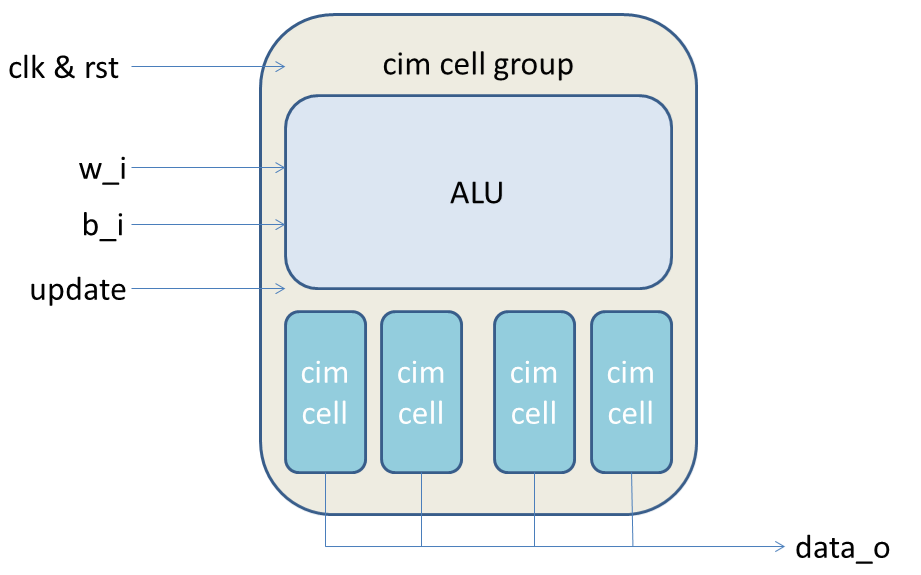
\includegraphics[width=0.8\textwidth]{ccg.png}
	\caption{cim\_cell\_group模块简图}
	\label{ccg}
\end{figure}
\subsection{端口说明}
\subsubsection{IN}
\begin{itemize}
	\item \textbf{clk \& rst}: external signals. 固有信号,系统时钟与系统重置信号。
	\item \textbf{w\_i}: 输入的权重,作为ALU的输入。
	\item \textbf{b\_i}: 输入的待运算数据,作为ALU的输入。
	\item \textbf{update}: 更新信号,指示cim\_cell进行累加操作,具体cim\_cell编号依据内部计数器(count)决定。
\end{itemize}
\subsubsection{OUT}
\begin{itemize}
	\item \textbf{data\_o}: 输出cim\_cell内部数据,以数组的形式。
\end{itemize}

\section{cim\_cell}
\subsection{模块简图}
cim\_cell\_group设计简图如图\ref{cimCell}所示。
\begin{figure}[htbp]
	\centering
	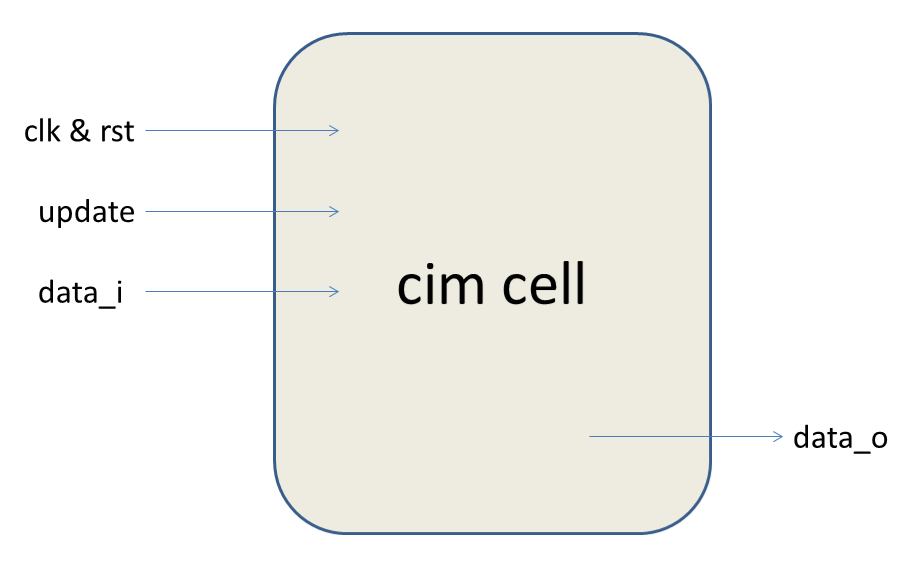
\includegraphics[width=0.8\textwidth]{cimCell.png}
	\caption{cim\_cell模块简图}
	\label{cimCell}
\end{figure}
\subsection{端口说明}
\subsubsection{IN}
\begin{itemize}
	\item \textbf{clk \& rst}: external signals. 固有信号,系统时钟与系统重置信号。
	\item \textbf{data\_i}: 输入的数据,待update信号为高电平与cim\_cell内部值相加更新原值。
	\item \textbf{update}: 更新信号,指示cim\_cell进行累加操作,具体cim\_cell编号依据内部计数器(count)决定。
\end{itemize}
\subsubsection{OUT}
\begin{itemize}
	\item \textbf{data\_o}: 输出cim\_cell内部数据。
\end{itemize}

\section{资源占用}
由于cim\_cell\_group(ccg)是可以参数化配置的,我们修改cim\_cell\_group的可配置参数\ref{params}(DATA\_WIDTH、N\_GROUP、ALU\_KIND)对其占用FPGA板载资源进行了较为丰富的实验\ref{expr}(暂不考虑Bonded IOB、BUFGCTRL资源)。ccg内部的ALU主要受ALU\_KIND、DATA\_WIDTH参数影响,cim\_cell主要受DATA\_WIDTH、N\_GROUP参数影响。
\begin{itemize}
	\label{params}
	\item \textbf{DATA\_WIDTH}: cim\_cell内部数据的宽度,单位是bit。
	\item \textbf{N\_GROUP}: cim\_cell\_group内部包含cim\_cell的数量。
	\item \textbf{ALU\_KIND}: cim\_cell\_group内部ALU的运算行为。当值为0时,ALU进行XNOR运算;当值为1时,ALU进行MUL运算。
\end{itemize}
\begin{table}[!hpb]
	\center
	\caption{cim\_cell\_group板载资源占用实验}
	\label{expr}
	\begin{tabular}{|c|c|c|c|c|}
		\hline
		No. & <ALU\_KIND, DATA\_WIDTH, N\_GROUP> & Slice LUTs & Slice Registers & DSPs \\ \hline
		1 & <0, 32, 1> & 34/31/33 & 33/0/32 & 0/0/0\\ \hline
		2 & <1, 32, 1> & 49/15/33 & 33/0/32 & 3/3/0\\ \hline
		3 & <0, 32, 4> & 134/124/33 & 131/0/32 & 0/0/0\\ \hline
		4 & <1, 32, 4> & 149/15/33 & 131/0/32 & 3/3/0\\ \hline
		5 & <0, 32, 12> & 401/372/33 & 389/0/32 & 0/0/0\\ \hline
		6 & <1, 32, 12> & 416/15/33 & 389/0/32 & 3/3/0\\ \hline
		7 & <0, 32, 1024> & 33854/31744/33 & 389/0/32 & 0/0/0\\ \hline
		8 & <1, 32, 1024> & 33869/32783/1 & 32811/0/32 & 3/3/0\\ \hline
	\end{tabular}
\end{table}

\bibliographystyle{plain}
\bibliography{wpref}

\end{document}
